%% =============================================================================
%% SoftwareX submission — Original Software Publication
%% "Aetherion: A structure-preserving, differentiable C++23 library for
%%  six-degree-of-freedom flight dynamics"
%%
%% Author: Onur Tuncer, Istanbul Technical University
%%
%% Prepared with the SoftwareX article template (Version 4, November 2023),
%% which is based on Elsevier's `elsarticle' document class.
%%
%% Journal companion to the EUCASS library paper (papers/eucass-library) and to
%% the EUCASS integrator paper (papers/eucass).
%% =============================================================================

\documentclass[preprint,12pt,a4paper]{elsarticle}

\usepackage{amssymb}
\usepackage{amsmath}
\usepackage{graphicx}
\usepackage{booktabs}
\usepackage{subcaption}
\usepackage{listings}
\usepackage{xcolor}
\usepackage{siunitx}
\usepackage{float}
%% expansion=false: the template's title size resolves to a bitmap (pk) font,
%% and pdfTeX font expansion requires scalable fonts. Protrusion still applies.
\usepackage[expansion=false]{microtype}
\usepackage{hyperref}
%% Long \texttt{} identifiers (Spatial::Inertia, CppAD::AD<double>) cannot be
%% hyphenated; give TeX some slack rather than leaving overfull boxes.
\setlength{\emergencystretch}{2em}
%% The SoftwareX template zeroes \parindent; without a matching \parskip,
%% consecutive paragraphs run together visually.
\setlength{\parindent}{0pt}
\setlength{\parskip}{6pt}

%% ---------------------------------------------------------------------------
%% Listings style for C++
%% ---------------------------------------------------------------------------
\definecolor{lstkw}{HTML}{0F4C81}
\definecolor{lstcm}{HTML}{6B7280}
\definecolor{lstst}{HTML}{9A3412}
\definecolor{lstbg}{HTML}{F7F7F9}

\lstdefinestyle{cpp}{
  language=C++,
  basicstyle=\ttfamily\footnotesize,
  keywordstyle=\color{lstkw}\bfseries,
  commentstyle=\color{lstcm}\itshape,
  stringstyle=\color{lstst},
  backgroundcolor=\color{lstbg},
  frame=single,
  rulecolor=\color{lstcm!40},
  framesep=4pt,
  showstringspaces=false,
  columns=fullflexible,
  keepspaces=true,
  breaklines=true,
  captionpos=b,
  morekeywords={concept,requires,constexpr,consteval,noexcept,nullptr,auto,using,template,typename,struct,class,namespace}
}
\lstset{style=cpp}

%% ---------------------------------------------------------------------------
%% Math macros
%% ---------------------------------------------------------------------------
\newcommand{\SO}{\mathrm{SO}(3)}
\newcommand{\SE}{\mathrm{SE}(3)}
\newcommand{\se}{\mathfrak{se}(3)}
\newcommand{\Exp}{\mathrm{Exp}}
\newcommand{\dexp}{\mathrm{d}\exp}
\newcommand{\ad}{\mathrm{ad}}
\newcommand{\R}{\mathbb{R}}
\newcommand{\norm}[1]{\left\lVert #1 \right\rVert}
\newcommand{\nuB}{\boldsymbol{\nu}_B}
\newcommand{\IB}{\mathbf{I}_B}
\newcommand{\wext}{\mathbf{w}_{\mathrm{ext}}}
\newcommand{\code}[1]{\texttt{\small #1}}

\journal{SoftwareX}

\begin{document}

\begin{frontmatter}

\title{Aetherion: A structure-preserving, differentiable {C}++23 library for
       six-degree-of-freedom flight dynamics}

\author[label1]{Onur Tuncer\corref{cor1}}
\ead{otuncer@itu.edu.tr}
\cortext[cor1]{Corresponding author.}
\address[label1]{Department of Aerospace Engineering, Istanbul Technical
  University, Maslak, 34469 Istanbul, T\"urkiye}

\begin{abstract}
\textit{Six-degree-of-freedom (6-DOF) simulation underpins vehicle design,
control law verification and trajectory optimisation, but the codes used in
practice usually flatten the attitude state into an unconstrained array,
restore the constraint by periodic re-normalisation, and carry a second,
separately maintained implementation of the dynamics to obtain derivatives.
Aetherion removes all three by construction. The state is declared on the
product manifold $\SE \times \R^{7}$ and advanced by
Runge--Kutta--Munthe-Kaas (RKMK) integrators that never leave the group, so
orthonormality is exact rather than restored; all kinematics and dynamics are
expressed in Featherstone spatial vector algebra; and every model is a template
over the scalar type, so the differentiated code path \emph{is} the simulated
code path. Vehicles are assembled from gravity, aerodynamic, propulsion and
mass policies whose interfaces are C++20 concepts instantiated for both
\code{double} and an algorithmic-differentiation type, making AD-safety a
compile-time property. The library is verified against sixteen check cases from
NASA TM-2015-218675 and lies inside the envelope spanned by NASA's own
reference implementations in every case.}
\end{abstract}

\begin{keyword}
Flight dynamics \sep Geometric numerical integration \sep Lie group methods
\sep SE(3) \sep Algorithmic differentiation \sep Spatial vector algebra
\sep C++23
\end{keyword}

\end{frontmatter}

%% ---------------------------------------------------------------------------
\section*{Metadata}
\label{}
%% ---------------------------------------------------------------------------

\begin{table}[H]
\footnotesize
\begin{tabular}{|l|p{4.9cm}|p{6.9cm}|}
\hline
\textbf{Nr.} & \textbf{Code metadata description} & \textbf{Metadata} \\
\hline
C1 & Current code version & v0.12.0 \\
\hline
C2 & Permanent link to code/repository used for this code version &
     \url{https://github.com/onurtuncer/Aetherion} \\
\hline
C3 & Permanent link to Reproducible Capsule &
     Not applicable. All verification scenarios reported here are built and
     executed by the project's continuous integration workflows:
     \url{https://github.com/onurtuncer/Aetherion/actions} \\
\hline
C4 & Legal Code License & MIT License \\
\hline
C5 & Code versioning system used & git \\
\hline
C6 & Software code languages, tools, and services used &
     C++23; CMake; Python (post-processing and plotting scripts);
     GitHub Actions \\
\hline
C7 & Compilation requirements, operating environments \& dependencies &
     A C++23 compiler (GCC~13+, Clang~17+, or MSVC~19.38+) and CMake~3.26+.
     Dependencies: Eigen~3.4 (linear algebra), CppAD (algorithmic
     differentiation), nlohmann/json (configuration), Catch2 (tests),
     fmu4cpp (FMI export). Builds and is tested on Linux and Windows. \\
\hline
C8 & If available, link to developer documentation/manual &
     \url{https://onurtuncer.github.io/Aetherion/} \\
\hline
C9 & Support email for questions & \url{otuncer@itu.edu.tr} \\
\hline
\end{tabular}
\caption{Code metadata (mandatory)}
\label{codeMetadata}
\end{table}

\newpage

%% ---------------------------------------------------------------------------
\section{Motivation and significance}
\label{sec:motivation}
%% ---------------------------------------------------------------------------

The equations of motion of a rigid aerospace vehicle are not in dispute. What
differs between simulation codes---and what determines whether a code can be
reused, differentiated, verified, or trusted at the margins of its
envelope---is how those equations are \emph{expressed} in software. Three
recurring choices in existing 6-DOF codes motivated this work.

\textbf{Flattened state vectors.} The dominant idiom packs attitude, position,
velocity and mass into a single flat array and hands it to a general-purpose
ODE solver. This is convenient and wrong in a specific way: the attitude
components are constrained---a unit quaternion, or an orthonormal matrix---and
the solver does not know it. The constraint is then restored by periodic
re-normalisation, an ad hoc projection applied outside the integrator that
perturbs the trajectory and is invisible to any propagation Jacobian derived
from the solver. For a pure simulation this is often tolerable; for a filter or
an optimiser that consumes the solver's Jacobian, it is a silent modelling
error.

\textbf{Hand-written Jacobians.} Codes intended for estimation or optimisation
typically carry a second, separately maintained implementation of the dynamics
that returns partial derivatives. The two implementations drift apart. The
alternative---finite differences---introduces truncation error precisely where
the Newton or filter update is most sensitive to it.

\textbf{Vehicle-specific plumbing.} Aerodynamic, propulsion and mass models are
often hard-wired into the integration loop, so adding a vehicle means editing
the solver rather than supplying a model.

Existing open-source software addresses parts of this but is stratified by
purpose. JSBSim~\cite{berndt2004jsbsim} is a mature atmospheric flight dynamics
model with an extensive XML vehicle description format, oriented towards flight
simulation rather than towards differentiability or launch-vehicle
trajectories. General multibody libraries such as RBDL~\cite{felis2017rbdl} and
Pinocchio~\cite{carpentier2019pinocchio} implement Featherstone's algorithms
with high quality---Pinocchio in particular offers analytical
derivatives---but target robotic articulated systems and carry no atmosphere,
gravity-field or launch-vehicle staging models. On the geometry side, manif
\cite{deray2020manif} and comparable packages provide Lie group primitives with
Jacobians, but are libraries of group operations rather than of vehicle
dynamics. MATLAB's Aerospace Blockset and NASA's Trick and POST families are
widely used in industry but are respectively commercial and export-controlled
or distribution-restricted.

Aetherion occupies the intersection: aerospace vehicle models---US Standard
Atmosphere 1976~\cite{usstd1976}, WGS84 gravity~\cite{nima2000wgs84}, DAVE-ML
aerodynamic tables~\cite{jackson2002daveml}, multi-stage
propulsion---expressed in Featherstone spatial algebra, integrated by Lie-group
methods, and differentiable end-to-end through a single source. It is written
for researchers who need a 6-DOF plant that can be trusted numerically
\emph{and} handed to a gradient-based algorithm without being rewritten.

Two conference papers accompany this article and are referred to below where
relevant: a library overview~\cite{tuncer2027library} and a detailed treatment
of the implicit $\SE$ RKMK integrator and its Newton/AD
machinery~\cite{tuncer2027rkmk}. The present article is the software
publication: it describes what the library does, how it is put together, and
what has been verified, rather than deriving the numerics.

%% ---------------------------------------------------------------------------
\section{Software description}
\label{sec:description}
%% ---------------------------------------------------------------------------

Aetherion is a header-dominant C++23 library of roughly \num{40000} lines. Its
design rests on three commitments, each of which is enforced by the type system
rather than by convention.

\subsection{Software architecture}
\label{sec:architecture}

\textbf{One vocabulary: spatial vector algebra.} All kinematic and dynamic
quantities are 6-vectors in Featherstone's spatial
algebra~\cite{featherstone2008rbd}: twists
$\nuB = [\boldsymbol{\omega}_B^\top, \mathbf{v}_B^\top]^\top$, wrenches
$\mathbf{w} = [\mathbf{m}^\top, \mathbf{f}^\top]^\top$, the $6\times6$ spatial
inertia $\IB$, and the motion and force cross-product operators $\ad$ and
$\ad^*$. The equation of motion is then a single line,
\begin{equation}
  \IB(m)\,\dot{\nuB} + \ad^*(\nuB)\,\IB(m)\,\nuB = \wext,
  \label{eq:newton_euler}
\end{equation}
with no separate force and moment bookkeeping and no frame-specific special
cases. The types are distinct at compile time (\code{Spatial::Twist},
\code{Spatial::Wrench}, \code{Spatial::Inertia}), so a wrench cannot be
silently passed where a twist is expected.

\textbf{The state lives on the manifold.} The 6-DOF state is the triple
$(g, \nuB, m)$ on $\mathcal{M} = \SE \times \R^{6} \times \R_{>0}$, represented
as a pose $g \in \SE$ plus a Euclidean vector
$x = [\nuB^\top, m]^\top \in \R^{7}$. The two factors are advanced by different
retractions: $x$ by ordinary weighted sums, $g$ by the Lie exponential. Because
$g$ is only ever updated as $g \leftarrow g\,\Exp(\Delta)$ with $\Delta \in
\se$, the rotation factor is a product of exact $\SO$ elements and never needs
re-orthonormalisation. Aetherion treats the pose as a single $\SE$ element
rather than as a split $\SO \times \R^3$ product, so the screw coupling between
rotation and translation is retained.

\textbf{Scalar-type genericity.} Every model---gravity, atmosphere, table
interpolation, propulsion, the exponential map, the $\dexp^{-1}$ operator, the
Newton--Euler right-hand side---is a template over a scalar type $S$.
Instantiating with $S =$ \code{double} yields the simulation path; instantiating
with $S =$ \code{CppAD::AD<double>}~\cite{cppad} yields a differentiable path
through \emph{the same source}. There is no second implementation to keep in
step. This has a practical cost that shapes the code: branches on
floating-point comparisons do not tape correctly, so environment models are
written branch-free where possible and otherwise use conditional-expression
wrappers, and table lookups are interpolated with AD-transparent arithmetic
rather than with index-selecting control flow.

A vehicle is a composition of four policies---gravity, aerodynamics,
propulsion, mass---whose interfaces are C++20 concepts. The load-bearing detail
is that each concept is required to hold for \emph{both} scalar types:

\begin{lstlisting}[caption={Policy concepts are instantiated for \code{double} and for the AD type, so a model that is not differentiable is a compile error rather than a wrong Jacobian at run time.}, label={lst:concepts}]
template<class P, class S>
concept GravityPolicyFor =
    requires(const P& p, const Lie::SE3<S>& g, S mass) {
        { p(g, mass) } -> std::same_as<Spatial::Wrench<S>>;
    };

template<class P>
concept GravityPolicy =
       detail::GravityPolicyFor<P, double>
    && detail::GravityPolicyFor<P, CppAD::AD<double>>;
\end{lstlisting}

A policy that inadvertently applies \code{std::sqrt} to a raw \code{double}, or
takes a branch the tape cannot record, fails the concept check at the point of
use with a readable diagnostic---rather than producing a silently wrong
Jacobian at run time. Table~\ref{tab:modules} maps the modules; namespaces
mirror the directory structure.

\begin{table}[!h]
  \centering
  \caption{Module map.}
  \label{tab:modules}
  \footnotesize
  \begin{tabular}{@{}lp{8.4cm}@{}}
    \toprule
    Module & Responsibility \\
    \midrule
    \code{Spatial}        & Twists, wrenches, spatial inertia, $\ad$/$\ad^*$, transforms \\
    \code{ODE::RKMK::Lie} & $\SO$, $\SE$, $\Exp$, $\dexp^{-1}$, adjoints \\
    \code{ODE::RKMK::Core} & Butcher tableaux, stage residuals, Newton solve, AD Jacobian \\
    \code{ODE::RKMK::Integrators} & Radau IIA and explicit RK4 RKMK steppers \\
    \code{RigidBody}      & State, spatial inertia assembly, vector field, 6-DOF stepper \\
    \code{Environment}    & US1976 atmosphere, WGS84 gravity and constants, wind models \\
    \code{Aerodynamics}   & Aerodynamic angles, Mach number, force/moment assembly \\
    \code{Coordinate}     & ECI/ECEF/geodetic/NED conversions \\
    \code{FlightDynamics} & Gravity/aero/propulsion/mass policies, trim solver \\
    \code{Serialization}  & DAVE-ML model reader, JSON configuration \\
    \code{Simulation}     & Application template method, simulator interface, CSV snapshots \\
    \code{FMU}            & FMI 2.0/3.0 export wrappers \\
    \code{Examples}       & The sixteen verification scenarios \\
    \bottomrule
  \end{tabular}
\end{table}

The stage system, the residual and the Newton Jacobian are fixed-size Eigen
objects and are therefore stack-resident. No heap allocation occurs inside the
integration hot path other than the vector round-trips mandated by the CppAD
tape interface---a prerequisite for the real-time and hardware-in-the-loop use
the library is intended to support.

\subsection{Software functionalities}
\label{sec:functionalities}

\textbf{Lie-group integration.} RKMK methods~\cite{muntheKaas1998,
iserles2000liegroup, hairerLubichWanner2006gni} perform all Runge--Kutta stages
inside the Lie algebra---a vector space---and map back to the group with the
exponential. Two integrators are provided: a three-stage Radau~IIA scheme
(order~5, stiffly accurate, solved by Newton iteration with an exact CppAD
Jacobian) and an explicit four-stage RK4 scheme for cheap or non-stiff cases.
Both share the same stage residual formulation and the same $\Exp$/$\dexp^{-1}$
primitives. Any type satisfying the \code{LieGroup} concept---which requires
only \code{Identity}, composition, \code{Exp} and \code{dexp\_inv}---can be
substituted for $\SE$ without touching the stage machinery.

\textbf{Environment and vehicle models.} The US Standard Atmosphere 1976 is
implemented over the full layered profile in branch-free form; WGS84 constants
and an oblateness ($J_2$) gravity model are provided together with the full set
of ECI/ECEF/geodetic/NED conversions, whose round-trip consistency is
unit-tested over randomised inputs. Aerodynamic coefficients are read from
DAVE-ML model files~\cite{jackson2002daveml}---the same interchange format the
NASA reference cases are distributed in---and air-relative velocity accounts
for the rotating atmosphere, so aerodynamic angles are computed against the
moving air mass. Thrust and mass flow come from propulsion and mass policies;
staging is handled by event-triggered replacement of the active policies, with
per-stage propellant tracking and a centre-of-gravity offset that travels as
propellant is consumed.

\textbf{Trim.} A two-stage Newton--Raphson trim solver finds the
$(\alpha, \delta_e, \text{throttle})$ balancing a straight-and-level condition,
using an exact CppAD Jacobian for the longitudinal $2\times2$ subproblem and a
bisection inversion of the propulsion map for thrust.

\textbf{Interoperability.} Plants are exported as FMI 2.0 and 3.0 functional
mock-up units through fmu4cpp~\cite{fmu4cpp}, so an Aetherion vehicle can be
dropped into any FMI-compliant co-simulation environment; exported units
include the dragless sphere, the F-16 plant, an F-16 autopilot and the
two-stage rocket. Round-trip behaviour is smoke-tested in continuous
integration against the ecos co-simulation engine~\cite{ecos}, and Simulink
import is exercised by a dedicated workflow. Initial conditions and simulation
parameters are JSON; output is CSV in a column layout selectable at compile
time through \code{SnapshotTraits}, including a 31-column layout matching the
NASA reference files exactly so that comparison requires no column mapping.

%% ---------------------------------------------------------------------------
\section{Illustrative examples}
\label{sec:examples}
%% ---------------------------------------------------------------------------

\subsection{Defining and propagating a vehicle}

The composition of a vehicle is visible in its type. A vehicle's right-hand
side is a \code{VectorField} parameterised by its four policies; the stepper is
a \code{SixDoFStepper} parameterised by that vector field. The Newton--Euler
equation, the $\SE$ kinematics, the implicit stage system and the AD Jacobian
are all supplied by the library.

\begin{lstlisting}[caption={A complete vehicle definition and one integration step.}, label={lst:vehicle}]
using RocketVF = RigidBody::VectorField<
        RocketGravityPolicy,     // w_grav(g, m)
        RocketAeroPolicy,        // w_aero(g, nu_B, m, t)
        RocketPropulsionPolicy,  // w_prop(g, nu_B, m, t)
        RocketMassPolicy>;       // mdot(t, m)

using Stepper = RigidBody::SixDoFStepper<RocketVF>;  // Radau IIA RKMK, default

Stepper stepper{ inertialParameters, newtonOptions };

auto result = stepper.step(t, state, h);
if (result.converged)
    state = Stepper::unpack(result);
\end{lstlisting}

Substituting a different integrator is a third template argument; substituting
a different vehicle is four different policy types. Neither requires touching
the solver. A user-supplied policy needs only an \code{operator()} templated
over the scalar type; the recommended idiom is to follow its definition with
\code{static\_assert(FlightDynamics::GravityPolicy<MyPolicy>)}, which reports a
violation at the definition site rather than inside an integrator
instantiation.

\subsection{Convergence order and constraint preservation}

Order is verified rather than asserted, and the test problem is chosen so that
it can actually measure order. A torque-free \emph{symmetric} body is
degenerate for this purpose: its body twist is constant, the exact flow is a
one-parameter subgroup, and \emph{any} RKMK method reproduces it exactly at
every step size. The convergence study therefore uses a torque-free
\emph{asymmetric} rigid body ($I_{xx}, I_{yy}, I_{zz}$ all distinct) with
non-zero initial body velocity, so that Euler's equations are nonlinear, the
body twist genuinely varies, and the translational screw coupling is exercised.
Errors are measured against a reference computed at a step size 50 times
smaller than the finest tested step, cross-validated between the two
independent integrators.

Figure~\ref{fig:convergence} shows the result: mean log--log slopes of 5.00
(attitude and position) for Radau~IIA RKMK and 3.91/3.98 for explicit RK4
RKMK. Figure~\ref{fig:drift} shows the orthonormality residual
$\norm{R^\top R - I}_F$ over a \SI{600}{\second} tumbling trajectory. The
$\SE$ RKMK pose holds the constraint at $\sim$\num{4.4e-14} with no secular
growth, because the rotation factor is a product of exact $\SO$ elements; an
unconstrained quaternion RK4 state drifts to $\sim$\num{2.1e-3}. Per-step
re-normalisation of that quaternion does restore the constraint, to
$\sim$\num{6.9e-16}. The distinction is therefore not \emph{whether}
orthonormality is achieved but \emph{how}: re-normalisation is a projection
applied outside the integrator, which perturbs the solution and is not
represented in any propagation Jacobian derived from the solver.

\begin{figure}[!ht]
  \centering
  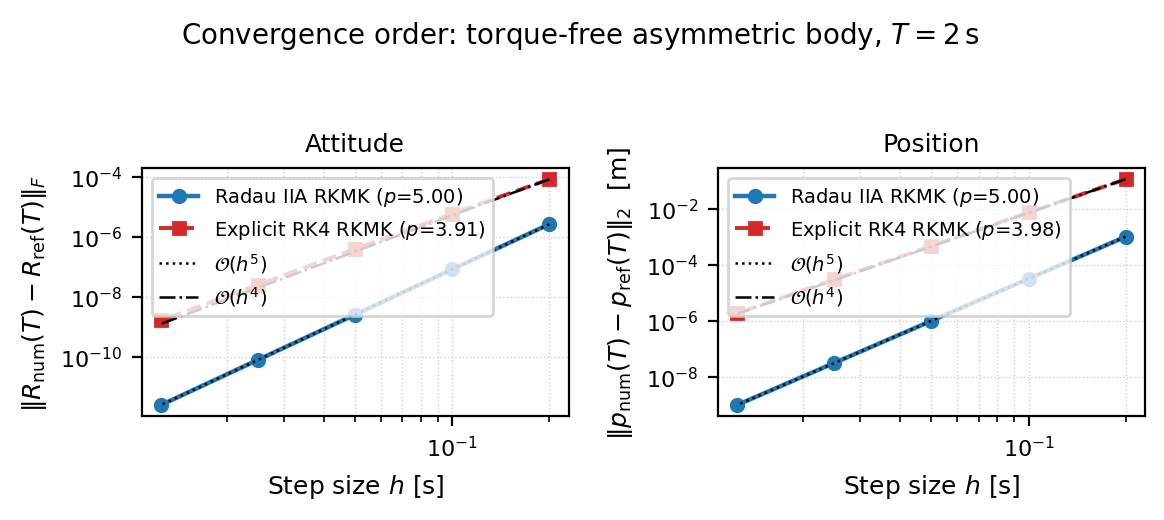
\includegraphics[width=\textwidth]{figures/convergence_order}
  \caption{Empirical convergence order: error against a fine-step reference at
    $T = \SI{2}{\second}$ for a torque-free asymmetric body. Mean log--log
    slopes are 5.00 (attitude and position) for Radau~IIA RKMK and 3.91/3.98
    for explicit RK4 RKMK. The study is a regression test in the suite and
    emits the data plotted here.}
  \label{fig:convergence}
\end{figure}

\begin{figure}[!ht]
  \centering
  
\includegraphics[width=0.8\textwidth]{figures/constraint_drift}
  \caption{Attitude constraint residual $\norm{R^\top R - I}_F$ over a
    \SI{600}{\second} tumbling trajectory, for $\SE$ RKMK, plain quaternion
    RK4, and quaternion RK4 with per-step re-normalisation.}
  \label{fig:drift}
\end{figure}

Both integrators additionally reproduce constant-twist motion \emph{exactly},
at every step size---the defining behaviour of a Lie-group method---and this is
asserted as a regression test.

\subsection{Verification against NASA reference trajectories}

NASA Technical Memorandum TM-2015-218675~\cite{NASA_TM_2015_218675} defines a
set of atmospheric and space flight check cases and publishes reference
trajectories generated by independently developed NASA simulation frameworks.
It is close to an ideal verification target: the vehicle models are fully
specified, the reference output is machine-readable, and the cases are graded
from analytically checkable point masses up to a full launch-vehicle ascent.
Aetherion implements sixteen of these cases as executable examples, each
writing a CSV file whose columns match the reference file exactly. The examples
are not toy drivers---they are the same code paths a user would write, and they
are built and run in continuous integration.

A single ``error against the reference'' number would be misleading here,
because the memorandum ships \emph{several} independent reference runs per
scenario---up to six---and those runs do not agree with each other. The useful
question is therefore not only how far Aetherion sits from one nominated
reference, but whether it sits inside the envelope the reference
implementations themselves span. Table~\ref{tab:verification} reports both.

\begin{table}[!h]
  \centering
  \caption{Verification against NASA TM-2015-218675. ``Aetherion'' is the
    maximum $\lvert\Delta h_{\mathrm{MSL}}\rvert$ against the closest NASA
    reference run over $0 < t \leq T$; ``NASA spread'' is the maximum
    disagreement among the NASA runs themselves over the same interval. All
    values in metres. Cases 1--10 use $\Delta t = \SI{2}{\milli\second}$ and
    11--16 $\Delta t = \SI{10}{\milli\second}$.}
  \label{tab:verification}
  \footnotesize
  \begin{tabular}{cllrr}
    \toprule
    Case & Scenario & $T$ [s] & Aetherion [m] & NASA spread [m] \\
    \midrule
     1 & Dragless sphere              & 30  & $2.0\times10^{-5}$ & $7.1\times10^{-4}$ \\
     2 & Tumbling brick, undamped     & 30  & $2.0\times10^{-5}$ & $7.1\times10^{-4}$ \\
     3 & Tumbling brick, damped       & 30  & $2.0\times10^{-5}$ & $3.6\times10^{-4}$ \\
     6 & Sphere with drag             & 30  & $1.2\times10^{-5}$ & $0.273$ \\
     7 & Dropped sphere, steady wind  & 30  & $1.8\times10^{-5}$ & $0.273$ \\
     8 & Dropped sphere, wind shear   & 30  & $5.4\times10^{-5}$ & $0.273$ \\
     9 & Eastward cannonball          & 30  & $4.0\times10^{-4}$ & $1.30$ \\
    10 & Northward cannonball         & 30  & $1.8\times10^{-4}$ & $1.30$ \\
    11 & F-16 subsonic trim           & 180 & $13.2$  & $13.7$  \\
    12 & F-16 supersonic trim         & 180 & $97.5$  & $140$   \\
    13.1 & F-16 altitude change       & 180 & $0.171$ & $0.316$ \\
    13.2 & F-16 airspeed change       & 180 & $0.138$ & $1.21$  \\
    13.3 & F-16 heading change        & 180 & $0.178$ & $0.288$ \\
    13.4 & F-16 lateral side step     & 180 & $0.172$ & $0.295$ \\
    15 & F-16 polar circumnavigation  & 180 & $0.030$ & $0.430$ \\
    16 & F-16 equatorial circuit      & 180 & $0.036$ & $0.293$ \\
    \bottomrule
  \end{tabular}
\end{table}

In every case Aetherion lies within the envelope spanned by the NASA reference
implementations, and for the analytic and ballistic cases (1--10) it agrees
with the closest reference by one to four orders of magnitude more tightly than
those references agree with one another. For cases 6--10, where the NASA runs
disagree by \SIrange{0.27}{1.3}{\metre}, Aetherion tracks the closest run to
$\sim$\SI{e-5}{\metre}. This is the strongest statement the data supports: the
residual disagreement is dominated by differences among the reference
implementations, not by Aetherion. We report the maximum over the trajectory
rather than the endpoint value, and exclude $t = 0$, where the wind cases
differ by convention---the NASA files record true airspeed as exactly zero at
release, whereas Aetherion reports the air-relative speed, which is non-zero in
a crosswind.

A seventeenth scenario, a two-stage rocket ascent from sea level to
\SI{232}{\kilo\metre}, exercises the whole library at once: variable mass,
travelling centre of gravity, supersonic and hypersonic aerodynamic tables, and
staging. Through the first-stage burn the altitude error against the NASA
Sim~06 reference stays below \SI{0.15}{\percent} and the speed error below
\SI{1.5}{\metre\per\second}; the offset is unchanged through the coast phase,
confirming that the spatial inertia and gravity model are consistent in
ballistic flight. Two known modelling differences account for most of the
residual disagreement later in the trajectory and are stated rather than
absorbed into a tolerance: the variable-mass Newton--Euler equation strictly
carries an inertia-relief term $-\dot{\IB}\nuB$ that Aetherion currently
approximates by rebuilding $\IB$ from the fuel state each step, and the pitch
history during coast decays at a slightly different rate than the reference,
which shifts the effective second-stage ignition attitude.

%% ---------------------------------------------------------------------------
\section{Impact}
\label{sec:impact}
%% ---------------------------------------------------------------------------

Aetherion's contribution is that it makes several properties usually traded off
against one another available simultaneously, and makes them checkable.

\textbf{A differentiable 6-DOF plant that needs no second implementation.}
Gradient-based trajectory optimisation, parameter identification and
manifold-consistent state estimation all require derivatives of the dynamics.
The usual options are a hand-written Jacobian that drifts out of step with the
simulation, or finite differences whose truncation error is worst exactly where
the update is most sensitive. Because every Aetherion model is a template over
the scalar type and the concepts quantify over both instantiations, the
differentiated path is the simulated path by construction, and a model that is
not AD-safe fails to compile. This is the property that makes the library
usable as the plant inside an optimiser rather than only as a checker of one.

\textbf{Constraint preservation that survives linearisation.} Because the
attitude never leaves $\SO$, there is no projection step outside the
integrator, and the Jacobian the solver produces is the Jacobian of the map
that was actually applied. For an extended Kalman filter on the same product
manifold---the principal motivating application---this removes a well-known
source of inconsistency between the propagation model and its linearisation.

\textbf{An honest verification baseline.} The reference-spread methodology in
Section~\ref{sec:examples} is reusable independently of the library. Reporting
agreement against a single nominated reference run, when the published
references disagree with one another by more than the quantity being reported,
overstates what has been shown. Publishing both numbers side by side is a
better standard for the field, and the comparison tooling is part of the
repository.

\textbf{A reusable defect report.} The convergence study exposed a trivialisation
sign error that is easy to reproduce: the kinematic ODE is left-trivialised
($\dot g = g\hat\xi$), so with $g(t) = g_0\Exp(u(t))$ the stage correction is
$\dot u = \dexp^{-1}_{-u}(\xi)$ and must be evaluated at $-\eta_i$. Evaluating
at $+\eta_i$---the right-trivialised convention, and the form in which the
Bernoulli series is most often tabulated---flips the sign of the $O(\ad)$ term
and silently caps the method at order~2 for \emph{any} Butcher tableau. The
failure is invisible to the usual smoke tests: the pose stays exactly on
$\SE$, Newton still converges, and constant-twist motion is still integrated
exactly, because $\ad_\eta \eta = 0$ annihilates the offending term. It is
detected only by a convergence study on a problem with time-varying twist. Any
reader implementing RKMK is likely to reproduce this, and the companion
paper~\cite{tuncer2027rkmk} develops it in full.

The library is used by the author's group for launch-vehicle ascent studies and
control law verification, and is offered as a foundation for work in trajectory
optimisation, manifold-consistent state estimation and flight control
verification. FMI export means it can also serve as a high-fidelity plant
inside existing commercial co-simulation toolchains without adopting the C++
API at all.

For a library whose purpose is to be trusted numerically, process is part of
the contribution. The code base follows a practical subset of the JSF~AV C++
coding standard~\cite{jsfav2005}, with deviations documented individually
rather than waived silently. Every pull request runs Linux and Windows builds,
a Catch2 suite of approximately \num{590} test cases across 69 translation
units, AddressSanitizer and UndefinedBehaviorSanitizer, Clang-Tidy, IWYU
include hygiene, Clang-Format/CMake-Format/CMake-Lint, a Metrix++ cyclomatic
complexity budget, Codecov line coverage, the Simulink FMU import round trip,
and Doxygen and Sphinx documentation builds published to GitHub Pages. The
convergence-order and constraint-drift studies of Section~\ref{sec:examples}
are themselves regression tests, and they emit the data files from which
Figures~\ref{fig:convergence} and~\ref{fig:drift} are generated---so a change
that degrades the
integrator fails the build rather than quietly degrading a published claim.

%% ---------------------------------------------------------------------------
\section{Conclusions}
\label{sec:conclusions}
%% ---------------------------------------------------------------------------

Aetherion demonstrates that manifold correctness, differentiability,
extensibility and verifiability can be obtained simultaneously in 6-DOF flight
dynamics software if they are expressed in the type system rather than in
convention. The state is declared on $\SE \times \R^{7}$ and advanced by RKMK
integrators that keep it there, with convergence orders measured at 5.00 and
3.9 rather than assumed and the attitude constraint held at the round-off level
over \SI{600}{\second} trajectories. Every model is written once and evaluates
identically under \code{double} and under an AD type, with the requirement
enforced by concepts that quantify over both. Vehicles are compositions of four
policies, so adding one means writing models rather than editing the solver.
And the whole is verified against sixteen published NASA reference
trajectories, from analytic point masses to a two-stage ascent, with the
verification studies wired into continuous integration.

The library is at version~0.12 and is explicitly pre-1.0. Known gaps, rather
than design positions, are: the manifold extended Kalman filter that motivates
much of the architecture is currently a stub; the inertia-relief term
$-\dot{\IB}\nuB$ is approximated rather than carried explicitly; the
integrators are fixed-step, with an embedded Radau~IIA error estimate and
adaptive stepping planned; articulated multibody dynamics are not implemented,
although the spatial-algebra foundation is the standard one for it; and DAVE-ML
ingestion covers the subset exercised by the NASA check cases rather than the
complete specification. Source code, documentation and all verification
scenarios are available under the MIT licence~\cite{aetherion_2025}.

%% ---------------------------------------------------------------------------
\section*{Declaration of competing interest}
%% ---------------------------------------------------------------------------

The author declares that he has no known competing financial interests or
personal relationships that could have appeared to influence the work reported
in this paper.

%% ---------------------------------------------------------------------------
\section*{Acknowledgements}
%% ---------------------------------------------------------------------------

The author thanks the NASA Engineering and Safety Center (NESC) for making the
reference simulation data from TM-2015-218675 publicly available.

%% ---------------------------------------------------------------------------
\bibliographystyle{elsarticle-num}
\bibliography{references}

\end{document}
